\documentclass[conference,10pt,compsocconf]{IEEEtran}

% *** CITATION PACKAGES ***
%
\usepackage{cite}
% cite.sty was written by Donald Arseneau
% V1.6 and later of IEEEtran pre-defines the format of the cite.sty package
% \cite{} output to follow that of IEEE. Loading the cite package will
% result in citation numbers being automatically sorted and properly
% "compressed/ranged". e.g., [1], [9], [2], [7], [5], [6] without using
% cite.sty will become [1], [2], [5]--[7], [9] using cite.sty. cite.sty's
% \cite will automatically add leading space, if needed. Use cite.sty's
% noadjust option (cite.sty V3.8 and later) if you want to turn this off.
% cite.sty is already installed on most LaTeX systems. Be sure and use
% version 4.0 (2003-05-27) and later if using hyperref.sty. cite.sty does
% not currently provide for hyperlinked citations.
% The latest version can be obtained at:
% http://www.ctan.org/tex-archive/macros/latex/contrib/cite/
% The documentation is contained in the cite.sty file itself.
%
\usepackage{setspace}
\usepackage{wrapfig}
\usepackage{color}
\usepackage{balance}

%\usepackage[pdftex]{graphicx}
\usepackage{graphicx}
% declare the path(s) where your graphic files are
\graphicspath{{./}{./figs}}
% and their extensions so you won't have to specify these with
% every instance of \includegraphics
\DeclareGraphicsExtensions{.pdf,.jpeg,.png}

% *** SUBFIGURE PACKAGES ***
\usepackage[tight,footnotesize]{subfigure}
% \usepackage{subfigure}
% subfigure.sty was written by Steven Douglas Cochran. This package makes it
% easy to put subfigures in your figures. e.g., "Figure 1a and 1b". For IEEE
% work, it is a good idea to load it with the tight package option to reduce
% the amount of white space around the subfigures. subfigure.sty is already
% installed on most LaTeX systems. The latest version and documentation can
% be obtained at:
% http://www.ctan.org/tex-archive/obsolete/macros/latex/contrib/subfigure/
% subfigure.sty has been superceeded by subfig.sty.

%\usepackage[caption=false]{caption}
%\usepackage[font=footnotesize]{subfig}
% subfig.sty, also written by Steven Douglas Cochran, is the modern
% replacement for subfigure.sty. However, subfig.sty requires and
% automatically loads Axel Sommerfeldt's caption.sty which will override
% IEEEtran.cls handling of captions and this will result in nonIEEE style
% figure/table captions. To prevent this problem, be sure and preload
% caption.sty with its "caption=false" package option. This is will preserve
% IEEEtran.cls handing of captions. Version 1.3 (2005/06/28) and later
% (recommended due to many improvements over 1.2) of subfig.sty supports
% the caption=false option directly:
%\usepackage[caption=false,font=footnotesize]{subfig}
%
% The latest version and documentation can be obtained at:
% http://www.ctan.org/tex-archive/macros/latex/contrib/subfig/
% The latest version and documentation of caption.sty can be obtained at:
% http://www.ctan.org/tex-archive/macros/latex/contrib/caption/

% *** PDF, URL AND HYPERLINK PACKAGES ***
%
\usepackage{url}
% url.sty was written by Donald Arseneau. It provides better support for
% handling and breaking URLs. url.sty is already installed on most LaTeX
% systems. The latest version can be obtained at:
% http://www.ctan.org/tex-archive/macros/latex/contrib/misc/
% Read the url.sty source comments for usage information. Basically,
% \url{my_url_here}.

% *** Do not adjust lengths that control margins, column widths, etc. ***
% *** Do not use packages that alter fonts (such as pslatex).         ***
% There should be no need to do such things with IEEEtran.cls V1.6 and later.
% (Unless specifically asked to do so by the journal or conference you plan
% to submit to, of course. )

\begin{document}
\title{Optimizing Application Performance on a Burst Buffer using
Holistic I/O Characterization}

\maketitle

\begin{abstract}

\textcolor{red}{TODO: this abstract is already out of sync, likely to have
more emphasis on burst buffer at least.}

A variety of instrumentation and analysis tools have been utilized to
great effect to help understand and optimize components such as disk
arrays, file servers, libraries, and applications.  However, these
tools operate in isolation with a limited view of the system as a whole.
An integrated, holistic approach to I/O characterization is needed on
today's increasingly complex systems in order to fully understand
the interactions between components.  These complex interactions are what 
ultimately dictate overall scientific productivity in practice.

In this work we explore a case study in holistic I/O characterization
using an exemplar scientific computing application [description(s?)] on
Cori [description].  Our case study brings together characterization from
X,Y,Z to illustrate how [application performance?  system performance?]
could be improved via integrated holistic I/O characterization.
We make THING A go B \% faster for a meaningful workload.  We evaluate
our instrumentation methods and find that this approach is not only
highly valuable for case studies, but is also entirely feasible for
ongoing 24/7 production deployment without perturbing applications [some
empirical backup].  Finally, we propose a set of recommendations for
how this methodology can be automated in the future.

\end{abstract}

\section{Introduction}

I/O is hard and burst buffers are hard.

\section{NOTES}

This section is an attempt at transcribing notes from our ongoing email
discussions:

Our general approach is to run VPIC-IO on Cori, with and without using
burst buffers. We will collect data from the following sources:

\begin{itemize}
\item Darshan logs
\item LMT
\item SLURM job logs
\item DVS/Datawarp counters
\end{itemize}

We then gather the resulting logs into a centralized location and manually
look at how they fit together, determine gaps in the info each tool provides,
and determine which pieces of data have the most influence on I/O performance.

Open issues and notes:

\begin{itemize}
\item Retrieving both client-side and server-side Datawarp counters
    \begin{itemize}
    \item Glenn investigating quick/dirty way to grab raw counters out of Datawarp servers
    \item Glenn also investigating how to grab client side Datawarp counters
        \begin{itemize}
        \item Ideally, use a tool like procmon from NERSC to grab client-side data, but limited docs
        \item Currently just using a script that runs in parallel with VPIC-IO that gathers:
              number of writes, max write size, min write size for each compute node
        \end{itemize}
    \end{itemize}
\item Initial VPIC-IO job configurations:
    \begin{itemize}
    \item 2K and 16K core runs, each trying Lustre scratch FS vs burst buffer
    \item BB runs using 20 nodes for 2K runs, 87 nodes for 16K runs
    \item What are the striping parameters used for the scratch Lustre runs? Cori default?
    \end{itemize}
\item Breakdown of raw LMT data:
    \begin{itemize}
    \item For every 5s interval:
        \begin{itemize}
        \item For each OST: bytes read, bytes written, CPU \%
        \item For each MDS: frequency counts of a bunch of ops (opens, close, getattr, ...)
        \end{itemize}
    \item Contrast with Darshan data:
        \begin{itemize}
        \item Darshan only stores absolute time of job start and end times
        \item Darshan stores a few relative timestamps of first and last open/read/write/close ops
        \end{itemize}
    \item Phil: these things might be interesting to investigate further:
        \begin{itemize}
        \item correlate Darshan's observed I/O times with LMT data (currently aggregate LMT data,
              but could look at specific OSTs once we have access to that info)
        \item correlate amount of data moved according to LMT vs observed data movement in Darshan
              (again, initially looking at aggregate LMT, hopefully with ability to focus on OSTs later)
        \item correlate Darshan's discrete counts of file I/O ops (e.g., opens) to LMT data
        \end{itemize}
    \item Phil: Will we see flurry of LMT data at end of BB runs as data is staged out?
        \begin{itemize}
        \item Glenn: No, stage out happens after job and MPI processes are terminated -- will need to
              instrument BB nodes themselves to observe this activity, which Glenn is investigating
        \item Glenn: Further, stage out only happens when explicitly requested by the job script --
              does VPIC-IO explicitly flush the BB nodes?
        \end{itemize}
    \item Shane has some scripts for post-processing LMT data into a format that is more easily
          graphable, and made the following observations:
        \begin{itemize}
        \item CPU PCT is always 0 -- If we want to look at this metric, Glenn will need to find this
              data in another LMT table
        \item Some missing intervals in LMT data -- Glenn: LMT uses UDP and can drop packets, so
              keep this in mind when analyzing this data
        \end{itemize}
    \item Glenn: still need to grab LMT data for \textbf{after} the BB runs, since this is whe data
          is flushed to Lustre
    \end{itemize}
\item Incorporation of Lustre module into Darshan
    \begin{itemize}
    \item All: a Lustre module would be pretty useful...
    \item Shane has stubbed out Lustre module implementation he has shared with Glenn
        \begin{itemize}
        \item Need to determine lowest overhead way of getting data: /proc or liblustre API?
        \item Grab anything else besides: stripe params and OSTs associated with each file?
        \item If enabled, every file opened at the POSIX layer will be handed to the Lustre
              module to obtain Lustre data
        \item Glenn: stripe params and OST mappings are immutable, so these data records
              only need to be set once per file
        \end{itemize}
    \end{itemize}
\item Initial observations of VPIC-IO runs:
    \begin{itemize}
    \item Glenn: every proc is opening the file, though only 1/3 are writing. Could the
          low BB performance be due to the large metadata workload?
        \begin{itemize}
        \item Phil: compare ratio of I/O to metadata time for the Lustre runs and the BB
              runs to confirm
        \item Phil: MPI-IO hints can be used to force only aggregators to open files
        \item Phil: is collective buffering even needed for burst buffers? Does increasing
              aggregators generally lead to better performance, or do we need to limit BB
              clients like we would try to do for a PFS
            \begin{itemize}
            \item Suren: has another fork of VPIC-IO which skirts H5Part and allows more control
                  over the underlying I/O -- we could use this to investigate the tuning of
                  collective I/O or to just use independent I/O
            \end{itemize}
        \item Suren: turns out metadata time is not significant in these runs, poor performance
              is probably due to something else
        \end{itemize}
    \item Suren: One of the 16K total MPI-IO writes is taking 27 seconds, which is about 15\%
          of the total I/O time
        \begin{itemize}
        \item This is not due to slow POSIX I/O (i.e., I/O to Lustre), so it's a skew or synchronization
              problem
        \item Suren: perhaps this is an issue with unbalanced aggregator workloads?
            \begin{itemize}
            \item All: we need to find out more specifically what each aggregator's workload looks like
            \item Shane: we could set DARSHAN\_DISABLE\_SHARED\_REDUCTIONS=1 in the environment to
                  get a basic understanding of the aggregator mapping and relative workloads
            \end{itemize}
        \end{itemize}
    \end{itemize}
\end{itemize}

\section{Methods}

We ran an example benchmark on Cori with and without burst buffer.

\subsection{I/O application benchmark (Suren)}

We ran Suren's application I/O benchmark, VPIC-IO.

\subsection{System description (Glenn)}

We used Cori, NERSC's Cray XC40 featuring 144 burst buffer nodes sprayed
across the dragonfly network.

\subsection{Data sources (Glenn)}

We collected data for the job time intervals from any sources we could think
of, including:

\begin{itemize}
\item Darshan~\cite{carns200924}
\item LMT
\item SLURM job log
\item hopefully some DVS metrics
\item ???
\end{itemize}

\section{Results}

We discovered many wonderful things.

\subsection{Application performance improvement on burst buffer}

This is where we put some pretty charts showing the performance comparison.
Also Phil's fourth bullet point:

\begin{itemize}
\item learn something interesting about the burst buffer and how it integrates
into the ecosystem
\end{itemize}

Initial figures showing correlation of LMT write traffic with Darshan's observed
write activity for the 2K and 16K runs directly to Lustre (no burst buffer) are
given in Figure~\ref{fig:2k-write} and Figure~\ref{fig:16k-write}, respectively.
I'm not sure these graphs currently meet the pretty requirement given above...

\begin{figure}
\centering
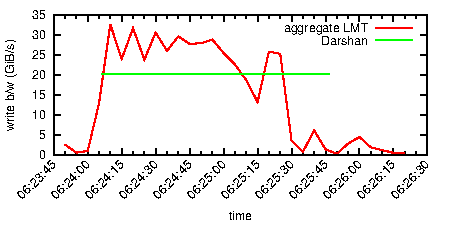
\includegraphics[width=0.5\textwidth]{figs/2k-lustre-wr-bw.pdf}
\caption{Correlating Darshan observed write interval and B/W with LMT's aggregate
write B/W for 2K VPIC run.}
\label{fig:2k-write}
\end{figure}

\begin{figure}
\centering
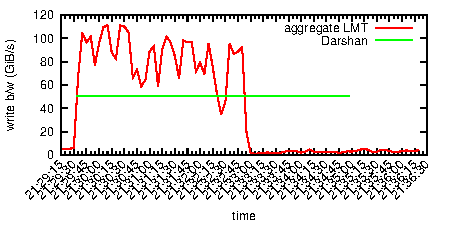
\includegraphics[width=0.5\textwidth]{figs/16k-lustre-wr-bw.pdf}
\caption{Correlating Darshan observed write interval and B/W with LMT's aggregate
write B/W for 16K VPIC run.}
\label{fig:16k-write}
\end{figure}

\subsection{Challenges in integrating data}

This will be more a methods section that calls out Phil's first two bullet points:

\begin{itemize}
\item identify gaps or things that need to be changed in one or more of the tools
to help make sense of the data
\item start getting ideas for how we would integrate the data in an automated
sense

We can also discuss the practicalities of extracting the leading factors
reflective of I/O performance (Jialin's idea).
\end{itemize}


\section{Conclusions}

We know a little more about I/O.

\bibliographystyle{IEEEtran}
\bibliography{REFERENCES}

\end{document}
